\documentclass[border=3mm]{standalone}
\usepackage{tikz}
\usetikzlibrary{arrows.meta,positioning,shapes.geometric,shapes.misc,fit,calc,backgrounds,decorations.pathreplacing}
\usepackage{amsmath,amssymb}

% Coordinated publication palette (accessible, high contrast, non-decorative)
\definecolor{colA}{HTML}{1A5276} % Slate Blue: Target Microservices
\definecolor{colB}{HTML}{922B21} % Deep Crimson: Security Chaos & Threats
\definecolor{colC}{HTML}{0E6655} % Deep Teal: RL Policy Controller
\definecolor{colD}{HTML}{B9770E} % Amber Ochre: Mitigation & Execution Queue
\definecolor{colE}{HTML}{1E8449} % Forest Green: Evaluation & SRE Metrics
\definecolor{bglight}{HTML}{FDFEFE}
\definecolor{linegray}{HTML}{34495E}

\begin{document}
\sffamily\footnotesize
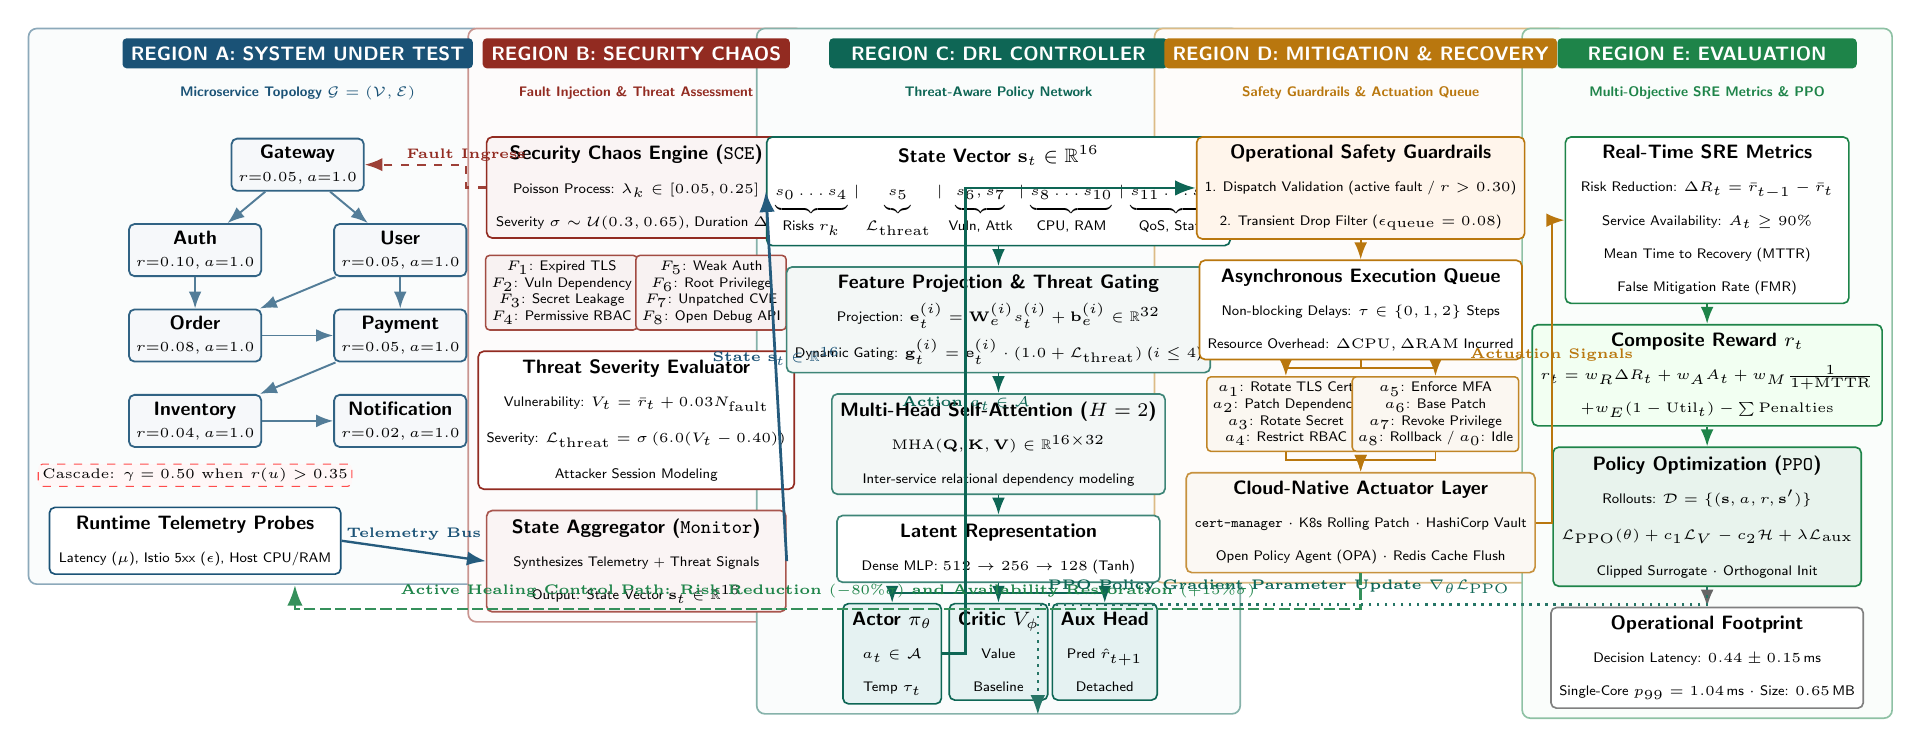
\begin{tikzpicture}[
    >=Latex,
    font=\sffamily,
    % Standard node styling
    boxnode/.style={
        draw=black!70, line width=0.6pt, fill=white,
        rounded corners=2pt, inner sep=3pt, align=center
    },
    svcnode/.style={
        draw=colA!90, line width=0.65pt, fill=colA!4,
        rounded corners=2pt, inner sep=2.5pt, minimum width=15mm, align=center,
        font=\sffamily\scriptsize
    },
    faultnode/.style={
        draw=colB!85, line width=0.55pt, fill=colB!6,
        rounded corners=1.5pt, inner sep=2pt, align=center,
        font=\sffamily\tiny
    },
    actionnode/.style={
        draw=colD!90, line width=0.55pt, fill=colD!6,
        rounded corners=1.5pt, inner sep=2pt, align=center,
        font=\sffamily\tiny
    },
    regheader/.style={
        font=\sffamily\bfseries\scriptsize, text=white,
        rounded corners=1.5pt, inner sep=3pt, align=center
    },
    regsub/.style={
        font=\sffamily\bfseries\tiny, align=center
    },
    % Arrow line styles
    flow/.style={
        ->, line width=0.7pt, draw=black!75
    },
    dataflow/.style={
        ->, line width=0.85pt, draw=colA!95
    },
    chaosflow/.style={
        ->, dashed, line width=0.75pt, draw=colB!90
    },
    healloop/.style={
        ->, line width=1.0pt, draw=colE!90, dash pattern=on 4pt off 1.5pt
    },
    learnloop/.style={
        ->, line width=0.9pt, draw=colC!90, dotted
    }
]

% ==============================================================================
% REGION A: SYSTEM UNDER TEST (MONITORED MICROSERVICES)
% ==============================================================================
\node[regheader, fill=colA, minimum width=37mm] (hdrA) at (0, 7.8) {REGION A: SYSTEM UNDER TEST};
\node[regsub, text=colA, below=1mm of hdrA] (subA) {Microservice Topology $\mathcal{G} = (\mathcal{V}, \mathcal{E})$};

% Microservice DAG Nodes
\node[svcnode, below=3.5mm of subA] (gw) {\textbf{Gateway}\\ \tiny $r{=}0.05, a{=}1.0$};
\node[svcnode, below left=4mm and -4mm of gw] (auth) {\textbf{Auth}\\ \tiny $r{=}0.10, a{=}1.0$};
\node[svcnode, below right=4mm and -4mm of gw] (user) {\textbf{User}\\ \tiny $r{=}0.05, a{=}1.0$};
\node[svcnode, below=4mm of auth] (order) {\textbf{Order}\\ \tiny $r{=}0.08, a{=}1.0$};
\node[svcnode, below=4mm of user] (pay) {\textbf{Payment}\\ \tiny $r{=}0.05, a{=}1.0$};
\node[svcnode, below=4mm of order] (inv) {\textbf{Inventory}\\ \tiny $r{=}0.04, a{=}1.0$};
\node[svcnode, below=4mm of pay] (notif) {\textbf{Notification}\\ \tiny $r{=}0.02, a{=}1.0$};

% Synchronous API Invocations
\draw[flow, draw=colA!75] (gw) -- (auth);
\draw[flow, draw=colA!75] (gw) -- (user);
\draw[flow, draw=colA!75] (auth) -- (order);
\draw[flow, draw=colA!75] (user) -- (order);
\draw[flow, draw=colA!75] (user) -- (pay);
\draw[flow, draw=colA!75] (order) -- (pay);
\draw[flow, draw=colA!75] (pay) -- (inv);
\draw[flow, draw=colA!75] (inv) -- (notif);

% Cascade Propagation Note
\node[draw=red!70, dashed, fill=red!3, rounded corners=1.5pt, inner sep=1.5pt, font=\tiny, below=2mm of inv] (cascade_note) 
    {Cascade: $\gamma=0.50$ when $r(u) > 0.35$};

% Telemetry Probes
\node[boxnode, draw=colA, fill=white, minimum width=37mm, below=2.5mm of cascade_note] (telemetry_probe) {
    \textbf{\scriptsize Runtime Telemetry Probes}\\
    \tiny Latency ($\mu$), Istio 5xx ($\epsilon$), Host CPU/RAM
};

% Region A Background Box
\begin{scope}[on background layer]
    \node[draw=colA!50, line width=0.6pt, fill=colA!2, rounded corners=3pt,
          fit=(hdrA) (subA) (gw) (notif) (cascade_note) (telemetry_probe)] (frameA) {};
\end{scope}

% ==============================================================================
% REGION B: SECURITY CHAOS & THREAT ASSESSMENT
% ==============================================================================
\node[regheader, fill=colB, minimum width=39mm] (hdrB) at (4.3, 7.8) {REGION B: SECURITY CHAOS};
\node[regsub, text=colB, below=1mm of hdrB] (subB) {Fault Injection \& Threat Assessment};

% Chaos Engine
\node[boxnode, draw=colB, fill=colB!5, minimum width=38mm, below=3.5mm of subB] (sce_engine) {
    \textbf{\scriptsize Security Chaos Engine (\texttt{SCE})}\\
    \tiny Poisson Process: $\lambda_k \in [0.05, 0.25]$\\
    \tiny Severity $\sigma \sim \mathcal{U}(0.3, 0.65)$, Duration $\Delta t$
};

% Standardized Fault Taxonomy (8 Faults)
\node[faultnode, below=2mm of sce_engine, xshift=-9.5mm, minimum width=18mm] (f_left) {
    $F_1$: Expired TLS\\
    $F_2$: Vuln Dependency\\
    $F_3$: Secret Leakage\\
    $F_4$: Permissive RBAC
};
\node[faultnode, below=2mm of sce_engine, xshift=9.5mm, minimum width=18mm] (f_right) {
    $F_5$: Weak Auth\\
    $F_6$: Root Privilege\\
    $F_7$: Unpatched CVE\\
    $F_8$: Open Debug API
};

% Threat Severity Assessment Module
\node[boxnode, draw=colB, fill=white, minimum width=38mm, below=2.5mm of f_left, xshift=9.5mm] (threat_eval) {
    \textbf{\scriptsize Threat Severity Evaluator}\\
    \tiny Vulnerability: $V_t = \bar{r}_t + 0.03 N_{\mathrm{fault}}$\\[1pt]
    \tiny Severity: $\mathcal{L}_{\mathrm{threat}} = \sigma\left(6.0(V_t - 0.40)\right)$\\[1pt]
    \tiny Attacker Session Modeling
};

% Observation Aggregator
\node[boxnode, draw=colB!80, fill=colB!5, minimum width=38mm, below=2.5mm of threat_eval] (obs_agg) {
    \textbf{\scriptsize State Aggregator (\texttt{Monitor})}\\
    \tiny Synthesizes Telemetry + Threat Signals\\
    \tiny Output: State Vector $\mathbf{s}_t \in \mathbb{R}^{16}$
};

% Region B Background Box
\begin{scope}[on background layer]
    \node[draw=colB!50, line width=0.6pt, fill=colB!2, rounded corners=3pt,
          fit=(hdrB) (subB) (sce_engine) (f_left) (threat_eval) (obs_agg)] (frameB) {};
\end{scope}

% ==============================================================================
% REGION C: THREAT-AWARE DEEP RL CONTROLLER
% ==============================================================================
\node[regheader, fill=colC, minimum width=43mm] (hdrC) at (8.9, 7.8) {REGION C: DRL CONTROLLER};
\node[regsub, text=colC, below=1mm of hdrC] (subC) {Threat-Aware Policy Network};

% State Vector Entry
\node[boxnode, draw=colC, fill=white, minimum width=41mm, below=3.5mm of subC] (ctrl_state) {
    \textbf{\scriptsize State Vector $\mathbf{s}_t \in \mathbb{R}^{16}$}\\
    \tiny $\underbrace{s_0 \dots s_4}_{\text{Risks } r_k} \mid \underbrace{s_5}_{\mathcal{L}_{\mathrm{threat}}} \mid \underbrace{s_6, s_7}_{\text{Vuln, Attk}} \mid \underbrace{s_8 \dots s_{10}}_{\text{CPU, RAM}} \mid \underbrace{s_{11} \dots s_{15}}_{\text{QoS, Status}}$
};

% Linear Feature Projection & Threat Gating
\node[boxnode, draw=colC!80, fill=colC!5, minimum width=41mm, below=2.5mm of ctrl_state] (ctrl_gate) {
    \textbf{\scriptsize Feature Projection \& Threat Gating}\\
    \tiny Projection: $\mathbf{e}_t^{(i)} = \mathbf{W}_e^{(i)} s_t^{(i)} + \mathbf{b}_e^{(i)} \in \mathbb{R}^{32}$\\[1pt]
    \tiny Dynamic Gating: $\mathbf{g}_t^{(i)} = \mathbf{e}_t^{(i)} \cdot (1.0 + \mathcal{L}_{\mathrm{threat}})$ ($i \le 4$)
};

% Multi-Head Self-Attention
\node[boxnode, draw=colC!80, fill=colC!5, minimum width=41mm, below=2.5mm of ctrl_gate] (ctrl_mhsa) {
    \textbf{\scriptsize Multi-Head Self-Attention ($H=2$)}\\
    \tiny $\mathrm{MHA}(\mathbf{Q}, \mathbf{K}, \mathbf{V}) \in \mathbb{R}^{16 \times 32}$\\
    \tiny Inter-service relational dependency modeling
};

% Dense Latent Layer
\node[boxnode, draw=colC!80, fill=white, minimum width=41mm, below=2.5mm of ctrl_mhsa] (ctrl_dense) {
    \textbf{\scriptsize Latent Representation}\\
    \tiny Dense MLP: $512 \to 256 \to 128$ (Tanh)
};

% Three Multi-Objective Decoupled Heads
\node[boxnode, draw=colC, fill=teal!10, below=2.5mm of ctrl_dense, xshift=-13.5mm, minimum width=12.5mm] (h_actor) {
    \textbf{\scriptsize Actor $\pi_\theta$}\\
    \tiny $a_t \in \mathcal{A}$\\
    \tiny Temp $\tau_t$
};
\node[boxnode, draw=colC, fill=teal!10, below=2.5mm of ctrl_dense, minimum width=12.5mm] (h_critic) {
    \textbf{\scriptsize Critic $V_\phi$}\\
    \tiny Value\\
    \tiny Baseline
};
\node[boxnode, draw=colC, fill=teal!10, below=2.5mm of ctrl_dense, xshift=13.5mm, minimum width=12.5mm] (h_aux) {
    \textbf{\scriptsize Aux Head}\\
    \tiny Pred $\hat{r}_{t+1}$\\
    \tiny Detached
};

% Connections inside Controller
\draw[flow, draw=colC] (ctrl_state) -- (ctrl_gate);
\draw[flow, draw=colC] (ctrl_gate) -- (ctrl_mhsa);
\draw[flow, draw=colC] (ctrl_mhsa) -- (ctrl_dense);
\draw[flow, draw=colC] (ctrl_dense.south) -- ++(0,-0.12) -| (h_actor.north);
\draw[flow, draw=colC] (ctrl_dense.south) -- (h_critic.north);
\draw[flow, draw=colC] (ctrl_dense.south) -- ++(0,-0.12) -| (h_aux.north);

% Region C Background Box
\begin{scope}[on background layer]
    \node[draw=colC!50, line width=0.6pt, fill=colC!2, rounded corners=3pt,
          fit=(hdrC) (subC) (ctrl_state) (ctrl_dense) (h_actor) (h_critic) (h_aux)] (frameC) {};
\end{scope}

% ==============================================================================
% REGION D: MITIGATION, QUEUE & RECOVERY
% ==============================================================================
\node[regheader, fill=colD, minimum width=40mm] (hdrD) at (13.5, 7.8) {REGION D: MITIGATION \& RECOVERY};
\node[regsub, text=colD, below=1mm of hdrD] (subD) {Safety Guardrails \& Actuation Queue};

% Operational Guardrails
\node[boxnode, draw=colD, fill=orange!8, minimum width=38mm, below=3.5mm of subD] (guard_box) {
    \textbf{\scriptsize Operational Safety Guardrails}\\
    \tiny 1. Dispatch Validation (active fault / $r > 0.30$)\\
    \tiny 2. Transient Drop Filter ($\epsilon_{\mathrm{queue}} = 0.08$)
};

% Asynchronous Execution Queue
\node[boxnode, draw=colD, fill=white, minimum width=38mm, below=2.5mm of guard_box] (queue_box) {
    \textbf{\scriptsize Asynchronous Execution Queue}\\
    \tiny Non-blocking Delays: $\tau \in \{0, 1, 2\}$ Steps\\
    \tiny Resource Overhead: $\Delta\mathrm{CPU}, \Delta\mathrm{RAM}$ Incurred
};

% Supported Remediation Actions (9 Actions)
\node[actionnode, below=2mm of queue_box, xshift=-9.5mm, minimum width=18mm] (act_left) {
    $a_1$: Rotate TLS Cert\\
    $a_2$: Patch Dependency\\
    $a_3$: Rotate Secret\\
    $a_4$: Restrict RBAC
};
\node[actionnode, below=2mm of queue_box, xshift=9.5mm, minimum width=18mm] (act_right) {
    $a_5$: Enforce MFA\\
    $a_6$: Base Patch\\
    $a_7$: Revoke Privilege\\
    $a_8$: Rollback / $a_0$: Idle
};

% Cloud-Native Actuation Layer
\node[boxnode, draw=colD!80, fill=colD!5, minimum width=38mm, below=2.5mm of act_left, xshift=9.5mm] (actuator_layer) {
    \textbf{\scriptsize Cloud-Native Actuator Layer}\\
    \tiny \texttt{cert-manager} $\cdot$ K8s Rolling Patch $\cdot$ HashiCorp Vault\\
    \tiny Open Policy Agent (OPA) $\cdot$ Redis Cache Flush
};

% Connections inside D
\draw[flow, draw=colD] (guard_box) -- (queue_box);
\draw[flow, draw=colD] (queue_box.south) -- ++(0,-0.1) -| (act_left.north);
\draw[flow, draw=colD] (queue_box.south) -- ++(0,-0.1) -| (act_right.north);
\draw[flow, draw=colD] (act_left.south) -- ++(0,-0.1) -| (actuator_layer.north);
\draw[flow, draw=colD] (act_right.south) -- ++(0,-0.1) -| (actuator_layer.north);

% Region D Background Box
\begin{scope}[on background layer]
    \node[draw=colD!50, line width=0.6pt, fill=colD!2, rounded corners=3pt,
          fit=(hdrD) (subD) (guard_box) (queue_box) (act_left) (act_right) (actuator_layer)] (frameD) {};
\end{scope}

% ==============================================================================
% REGION E: PERFORMANCE EVALUATION & RL FEEDBACK
% ==============================================================================
\node[regheader, fill=colE, minimum width=38mm] (hdrE) at (17.9, 7.8) {REGION E: EVALUATION};
\node[regsub, text=colE, below=1mm of hdrE] (subE) {Multi-Objective SRE Metrics \& PPO};

% SRE Real-Time Metrics
\node[boxnode, draw=colE, fill=white, minimum width=36mm, below=3.5mm of subE] (sre_metrics) {
    \textbf{\scriptsize Real-Time SRE Metrics}\\
    \tiny Risk Reduction: $\Delta R_t = \bar{r}_{t-1} - \bar{r}_t$\\
    \tiny Service Availability: $A_t \ge 90\%$\\
    \tiny Mean Time to Recovery (MTTR)\\
    \tiny False Mitigation Rate (FMR)
};

% Multi-Objective Reward Formulation
\node[boxnode, draw=colE, fill=green!5, minimum width=36mm, below=2.5mm of sre_metrics] (eval_reward) {
    \textbf{\scriptsize Composite Reward $r_t$}\\
    \tiny $r_t = w_R \Delta R_t + w_A A_t + w_M \frac{1}{1 + \mathrm{MTTR}}$\\
    \tiny $+ w_E (1 - \mathrm{Util}_t) - \sum \mathrm{Penalties}$
};

% PPO Policy Optimization Loop
\node[boxnode, draw=colE, fill=colE!10, minimum width=36mm, below=2.5mm of eval_reward] (eval_ppo) {
    \textbf{\scriptsize Policy Optimization (\texttt{PPO})}\\
    \tiny Rollouts: $\mathcal{D} = \{(\mathbf{s}, a, r, \mathbf{s}')\}$\\[1pt]
    \tiny $\mathcal{L}_{\mathrm{PPO}}(\theta) + c_1 \mathcal{L}_V - c_2 \mathcal{H} + \lambda \mathcal{L}_{\mathrm{aux}}$\\[1pt]
    \tiny Clipped Surrogate $\cdot$ Orthogonal Init
};

% Latency & Profile
\node[boxnode, draw=black!50, fill=white, minimum width=36mm, below=2.5mm of eval_ppo] (eval_profile) {
    \textbf{\scriptsize Operational Footprint}\\
    \tiny Decision Latency: $0.44 \pm 0.15$\,ms\\
    \tiny Single-Core $p_{99} = 1.04$\,ms $\cdot$ Size: $0.65$\,MB
};

% Connections inside E
\draw[flow, draw=colE] (sre_metrics) -- (eval_reward);
\draw[flow, draw=colE] (eval_reward) -- (eval_ppo);
\draw[flow, draw=black!60] (eval_ppo) -- (eval_profile);

% Region E Background Box
\begin{scope}[on background layer]
    \node[draw=colE!50, line width=0.6pt, fill=colE!2, rounded corners=3pt,
          fit=(hdrE) (subE) (sre_metrics) (eval_reward) (eval_ppo) (eval_profile)] (frameE) {};
\end{scope}

% ==============================================================================
% INTER-REGION FLOW ARROWS (DATA & CONTROL BUS)
% ==============================================================================

% 1. Chaos Disturbance Injection: SCE (Region B) -> Targeted Services in Region A
\draw[chaosflow] (sce_engine.west) -- ++(-0.25, 0) |- (gw.east)
    node[pos=0.35, above, font=\tiny\bfseries, text=colB] {Fault Ingress};

% 2. Telemetry Ingestion: Probes (Region A) -> State Aggregator (Region B)
\draw[dataflow] (telemetry_probe.east) -- (obs_agg.west)
    node[pos=0.5, above, font=\tiny\bfseries, text=colA] {Telemetry Bus};

% 3. Observation Stream: State Aggregator (Region B) -> State Vector (Region C)
\draw[dataflow, line width=1.0pt] (obs_agg.east) -- (ctrl_state.west)
    node[pos=0.5, above, font=\tiny\bfseries, text=colA] {State $\mathbf{s}_t \in \mathbb{R}^{16}$};

% 4. Action Dispatch: Actor Head (Region C) -> Safety Guardrails (Region D)
\draw[flow, draw=colC, line width=1.0pt] (h_actor.east) -- ++(0.3, 0) |- (guard_box.west)
    node[pos=0.25, above, font=\tiny\bfseries, text=colC] {Action $a_t \in \mathcal{A}$};

% 5. Actuation Telemetry: Actuators (Region D) -> SRE Metrics (Region E)
\draw[flow, draw=colD, line width=0.8pt] (actuator_layer.east) -- ++(0.2, 0) |- (sre_metrics.west)
    node[pos=0.25, above, font=\tiny\bfseries, text=colD] {Actuation Signals};

% 6. Active Healing Control Loop: Actuator Layer (Region D) -> Microservices (Region A)
% Routes cleanly beneath the diagram
\draw[healloop] (actuator_layer.south) -- ++(0, -0.45) -| ($(frameA.south) + (0.5, 0)$)
    node[pos=0.25, above, font=\tiny\bfseries, text=colE] {Active Healing Control Path: Risk Reduction $(-80\%\sigma)$ and Availability Restoration $(+15\%\sigma)$};

% 7. Closed-Loop Adaptation / Learning Loop: PPO (Region E) -> Controller (Region C)
% Routes cleanly beneath Region E and D to Region C
\draw[learnloop] (eval_ppo.south) -- ++(0, -0.22) -| ($(frameC.south) + (0.5, 0)$)
    node[pos=0.32, above, font=\tiny\bfseries, text=colC] {PPO Policy Gradient Parameter Update $\nabla_\theta \mathcal{L}_{\mathrm{PPO}}$};

\end{tikzpicture}
\end{document}
